\documentclass[11pt]{article}
\usepackage[margin=1in]{geometry}
\usepackage{amsmath,amssymb,amsthm,mathtools}
\usepackage{graphicx}
\usepackage{booktabs}
\usepackage{array}
\usepackage{placeins}
\usepackage[hyphens]{url}
\usepackage{microtype}
\usepackage{xcolor}
\usepackage[colorlinks=true,linkcolor=blue!55!black,citecolor=blue!55!black,urlcolor=blue!55!black]{hyperref}

\newcommand{\Tr}{\operatorname{Tr}}
\newcommand{\PB}{P_{\mathrm B}}
\newcommand{\Var}{\operatorname{Var}}
\newcommand{\ket}[1]{\lvert #1\rangle}
\newcommand{\bra}[1]{\langle #1\rvert}
\newcommand{\Np}{N'}
\newcommand{\Bern}{\mathrm{Bern}}
\newcommand{\eS}{e^{S_0}}

% status tags
\definecolor{cest}{RGB}{30,90,160}
\definecolor{cder}{RGB}{20,120,70}
\definecolor{cnum}{RGB}{150,90,10}
\definecolor{cconj}{RGB}{160,40,40}
\newcommand{\tagbox}[2]{\textsf{\small\color{#1}[#2]}}
\newcommand{\EST}{\tagbox{cest}{literature}}
\newcommand{\DER}{\tagbox{cder}{derived}}
\newcommand{\NUM}{\tagbox{cnum}{numerical}}
\newcommand{\CONJ}{\tagbox{cconj}{conjecture}}
\newcommand{\INTERP}{\tagbox{cconj}{interpretation}}

\newtheorem{proposition}{Proposition}
\theoremstyle{remark}
\newtheorem*{remark}{Remark}

\title{\bf Checkpoint, 28 September 2026:\\ the BPS uplift decoder of $\mathcal N{=}2$ SYK ---\\
verified structure, its variance, and\\ deviation from freeness as nonzero-length wormholes}
\author{\texttt{syk\_gravity} project \\[2pt] \small Drafted by Claude for J.~Chryssanthacopoulos; code state: commit \texttt{081877d} + working tree}
\date{}

\emergencystretch=2em
\begin{document}
\maketitle

\begin{abstract}
\noindent
This note records where the project stands after the September 2026 audit and one day of follow-up work. It has
two parts.

\emph{Part I} restates the results about the uplift decoder $O=\PB(1-n_i)\PB$ of one-flavor $\mathcal N{=}2$ SYK
that survived the audit: exact structure, BPS dimensions, the Haar/Wachter \emph{null} model, and robust numerics. It
adds new checks: the charge-sector structure of the BPS space, and an exact index formula reproducing every
measured BPS dimension. It also summarizes a new numerical campaign that measured the ``chord invariants''
(free cumulants, crossing weights, six-letter words) of the decoder for $q=3$, $\Np\le16$ and $q=5$, $\Np\le17$.

\emph{Part II} is analytic.
\begin{itemize}\itemsep1pt
\item \textbf{The variance is a zero-energy two-point function.} The decoder variance is exactly the zero-energy
  two-point function of the neutral bilinear $n_i-\mu$ in a \emph{single} R-charge sector.
\item \textbf{The super-Schwarzian gets the structure but not the size.} We re-derive the super-Schwarzian
  (LMRS) answer from the zero-energy wavefunctions. It reproduces the parity and R-charge structure of the data
  with no free parameters, but overshoots the magnitude by 15--60\,\%. We trace this to the absence of a
  conformal window at $\Np\lesssim16$.
\item \textbf{The finite-$\lambda$ chord formula matches.} The double-scaled super-chord formula of Boruch, Lin
  and Yan~\cite{BLY}, evaluated at $\lambda=2p^2/\Np$ with no free parameters, reproduces the measured variance
  to about 2\,\% for $\Np=5\ldots16$.
\item \textbf{Freeness corresponds to the zero-length wormhole.} In that theory the Haar/Wachter value of the
  second free cumulant is exactly the contribution of the \emph{zero-length} supersymmetric wormhole. The
  deviation from freeness is the contribution of wormholes of nonzero length:
  \[
  r=a+\sum_{n\ge1}P_n\,q^{2\Delta n}.
  \]
\end{itemize}
Each statement is tagged as \EST, \DER, \NUM, \INTERP\ or \CONJ.
\end{abstract}

\tableofcontents

%=====================================================================
\section{Scope, status labels, and notation}
%=====================================================================

\paragraph{Status labels.}
\EST: stated in a primary paper in \path{papers/} (cited).
\DER: follows from stated inputs by the derivation shown, or checked here to machine precision.
\NUM: observation from exact numerics at the sizes available.
\INTERP\ / \CONJ: reading or hypothesis, not established.

\paragraph{Model.} One-flavor $\mathcal N{=}2$ SYK~\cite{FGMS,CV}: $\Np$ complex fermions and a $p$-body supercharge
$Q=\sum_{i_1<\dots<i_p}C_{i_1\dots i_p}\psi^{i_1}\cdots\psi^{i_p}$ with i.i.d.\ complex Gaussian couplings, and
$H=\{Q,Q^\dagger\}$. We use $p=q=\hat q=3$ unless stated. In the code, $Q$ acts as $\omega\wedge$ on
$\Lambda^P(\mathbb C^{\Np})$.
\begin{itemize}\itemsep1pt
\item $\Np$ is the size of the \emph{enlarged} theory (old size $N=\Np-1$), and $P=\lfloor \Np/2\rfloor$.
\item $D=\binom{\Np}{P}$ is the dimension of the charge sector. $B$ is the BPS subspace ($\ker Q\cap\ker Q^\dagger$) at
  charge $P$, $d=\dim B$, and $\PB$ its projector.
\item $a=d/D$ is the BPS fraction. $\tau=\Tr_B/d$.
\end{itemize}

\paragraph{Decoder.} $O=\PB\,\Pi\,\PB$ restricted to $B$, with $\Pi=1-n_i$ (the ``slot'' projector; $i=\Np-1$ is the
uplift decoder of~\cite{CV}). With i.i.d.\ couplings every mode is statistically equivalent, so we average over
several modes.
\begin{itemize}\itemsep1pt
\item Eigenvalues $\lambda\in[0,1]$ are squared cosines of principal angles between $B$ and the slot.
\item UV mean $b=\Tr_D\Pi/D=1-P/\Np$.
\item Central quantity:
\begin{equation}
r\;\equiv\;\frac{\Var(\lambda)}{b(1-b)}\,,\qquad \Var(\lambda)=\tau(O^2)-\tau(O)^2 .
\label{eq:rdef}
\end{equation}
$r$ is the fraction of the ``UV'' Bernoulli variance that survives BPS projection. $0\le r\le 1$.
\end{itemize}

%=====================================================================
\part*{Part I --- Verified structure and numerics}
\addcontentsline{toc}{part}{Part I --- Verified structure and numerics}
%=====================================================================

\section{The safe core of the audit}\label{sec:safe}

The audit (\path{docs/project_archaeology.md}, \path{research/notes/gravitational_dual_fragility_audit.md})
checked the earlier draft claim by claim. What survived:

\subsection{Exact structure}
\begin{enumerate}\itemsep2pt
\item \EST\ $0\preceq O\preceq 1$, with $\lambda=\cos^2$ of the principal angles; definition as in~\cite[eqs.~101--102]{CV}.
  The BPS projector has the Hodge form $\PB=1-QGQ^\dagger-Q^\dagger GQ$, with $G$ the Green's function on the
  non-BPS part.
\item \DER\ \emph{Exact atoms.} $\lambda=1$ eigenvectors are BPS states of the old theory in the ``empty'' copy that
  are annihilated by wedging with the new-mode couplings. $\lambda=0$ eigenvectors are the analogous states in the
  ``occupied'' copy. (Characterization in the audit; implemented in \path{src/protected_atoms.py}.)
  \NUM\ The atom fraction is $55.6\,\%$ ($N=8,9$), $32.9\,\%$ ($10,11$), $5.6\,\%$ ($12,13$) and $0$ ($14$--$16$).
  This is a monotone decay close to rank lower bounds, not a resonance.
\item \DER\ \emph{Mean and pairing.} The disorder-averaged mean is $\langle\lambda\rangle=b$ (exchangeability of
  modes plus $\sum_i n_i=P$). Per realization this holds only at even $\Np$, half filling, where particle--hole
  symmetry pairs $\lambda\leftrightarrow1-\lambda$.
\item \DER\ \emph{Sum rule.} On the charge-$P$ sector, $\sum_i(n_i-\mu)=0$. Hence the BPS-projected covariance of two
  different modes is exactly $c=-1/(\Np-1)$. Measured: $-0.250,-0.200,\ldots,-0.067$ for $\Np=5\ldots15$.
\end{enumerate}

\subsection{BPS dimensions and charge sectors}\label{sec:sectors}
\begin{enumerate}\itemsep2pt
\item \EST\ $d=2\cdot3^{\Np/2-1}$ (even $\Np$, $P=\Np/2$) and $d=3^{(\Np-1)/2}$ (odd $\Np$)~\cite{CV}.
\item \DER\ + verified. Fermion number fixes the R-charge. With $\psi$ carrying charge $1/p$ and $Q$ charge $1$,
\begin{equation}
j=\frac{P-\Np/2}{p}\quad\Rightarrow\quad j=0\ (\Np\text{ even}),\qquad j=-\tfrac16\ (\Np\text{ odd}).
\label{eq:jsector}
\end{equation}
So $B$ is a \emph{single} R-charge sector. Exact counts: even $\Np$ has BPS states only at $j=0,\pm\frac13$, with
dimensions $(54;27,27)$, $(162;81,81)$, $(486;243,243)$ for $\Np=8,10,12$. The ratio $d_{\pm1/3}/d_0=\tfrac12$ is
exactly $\cos(\pi/3)/\cos0$, as predicted by $\Tr P_j\propto\cos\pi j$~\cite[eq.~82]{LMRS}. Odd $\Np$ has
$j=\pm\frac16$.
\item \DER\ + verified. The refined-index formula~\cite[eq.~A.4]{BLY},
\begin{equation}
\frac{d_j}{2^{\Np}}=\frac1p\sum_{n=0}^{p-1}\sin^{\Np}\!\Big(\frac{\pi n}{p}\Big)\,e^{i\pi jp}\,e^{-2\pi i jn},\qquad|j|<\tfrac12,
\label{eq:index}
\end{equation}
reproduces \emph{every} measured BPS dimension in every sector $|j|<\frac12$ for $\Np\le16$ (index saturation;
test \path{tests/test_dssyk_n2.py}). The inverse Fourier transform resolves $j$ only mod 1, hence the restriction.
\end{enumerate}

\subsection{The Haar / Wachter null model}\label{sec:haar}
Replace $\PB$ by a Haar-random projector of the same rank. Free probability then predicts that the law of $O$ is
the \emph{free compression} of $\Bern(b)$ by a free projection of trace $a$: the Wachter (MANOVA) law.
\begin{itemize}\itemsep1pt
\item \EST\ (Nica--Speicher~\cite{NS}) Compressing a variable $x$ by a free projection $p$ of trace $t$ gives
  \begin{equation}
  \kappa_n(pxp)=t^{\,n-1}\,\kappa_n(x)\qquad\text{(free cumulants, computed in the compressed algebra)}.
  \label{eq:NS}
  \end{equation}
\item Consequence \DER: for the Haar null model, $\rho_n\equiv\kappa_n/\kappa_n^{\Bern(b)}=a^{n-1}$. In particular
  \begin{equation}
  r_{\rm Haar}=\rho_2=a .
  \label{eq:rhaar}
  \end{equation}
\item \DER\ (audit) Exact finite-$D$ Weingarten moments hold, e.g.\ $m_2=b[D^2(a+b-ab)-1]/(D^2-1)$, as does the
  genus-one resolvent $W_1(x)=-b(1-a)(1-b)\,x(x-1)/[(x-\lambda_-)(x-\lambda_+)]^{5/2}$ (checked through $k=5$ and $6$).
  These are properties of the \emph{null model}. The audit found that the earlier ``gravity = Weingarten genus
  expansion'' reading is not supported.
\item \NUM\ Our Haar runs reproduce~\eqref{eq:rhaar} and $\rho_{4,6}=a^{3,5}$ to three digits for $\Np\ge7$. This
  validates the numerical pipeline.
\end{itemize}

\subsection{Robust numerics}
\NUM\ Interior level statistics of $O$ are GUE ($\langle r_{\rm gap}\rangle=0.599\pm0.001$ at $\Np=12$~\cite{CV}).
The interior density is \emph{not} Wachter: mid-band weight is depleted about $2\times$ and moves to the walls. Of order
$10$--$15\,\%$ of the spectrum lies below the Wachter edge at $\Np=13$--$16$.

\subsection{Retracted}
From the earlier draft (details in the audit):
\begin{itemize}\itemsep1pt
\item the end-of-world-brane dual with $\eS=D$;
\item ``BPS projection trivializes the Schwarzian'';
\item ``crossing $=$ handle $\propto D^{-2}$'';
\item the self-energy formula for $O$;
\item the ``tail $=$ image of the near-BPS spectrum'' explanation;
\item the bordered-Toeplitz closed form.
\end{itemize}
The Kunisky--Chebyshev error identity~\cite{Kunisky} holds for \emph{any} pair of projections, so it is bookkeeping,
not evidence.

%=====================================================================
\section{Chord invariants of the decoder}\label{sec:campaign}
%=====================================================================

\paragraph{What was measured.} All quantities are exact linear algebra, per disorder realization
(\path{src/chord_invariants.py}; \path{research/notes/chord_invariants_2026-09-28.md}). For centered
operators $\hat A_i=\PB(\Pi_i-\mu)\PB$ with $v_i=\tau(\hat A_i^2)$:
\begin{itemize}\itemsep1pt
\item free cumulants $\kappa_n$ ($n\le6$) of $O$, and the ratios $\rho_n=\kappa_n/\kappa_n^{\Bern(b)}$;
\item the crossing weight $X=\tau(\hat A_i\hat A_j\hat A_i\hat A_j)/(v_iv_j)$ and the non-crossing factorization
  $F=\tau(\hat A_i\hat A_i\hat A_j\hat A_j)/(v_iv_j)$ for $i\neq j$;
\item all six-letter pair words, compared with $X^{\mathrm{cr}}$, where cr is the crossing number.
\end{itemize}
The fully crossing word $ijkijk$ discriminates between two rules: free compression predicts $X^2$ and a
single-parameter chord ($q$-Gaussian) rule predicts $X^3$. We quote $e_3=\ln w_3/\ln X$.

\begin{table}[h]
\centering\small
\begin{tabular}{@{}cc c c c c c c c@{}}
\toprule
$q$ & $\Np$ & model & $a$ & $r$ & $\rho_4$ \,($a^3$) & $X$ & $F$ & $e_3$\\
\midrule
3 & 10 & SYK & 0.643 & 0.746 & 0.435 (0.266) & 0.810 & 0.995 & $2.29\pm0.01$\\
3 & 12 & SYK & 0.526 & 0.687 & 0.348 (0.146) & 0.785 & 0.995 & $2.35\pm0.01$\\
3 & 14 & SYK & 0.425 & 0.642 & 0.290 (0.077) & 0.769 & 0.994 & $2.41\pm0.01$\\
3 & 16 & SYK & 0.340 & 0.601 & 0.245 (0.039) & 0.755 & 0.995 & $2.42\pm0.03$\\
3 & 16 & Haar & 0.340 & 0.340 & 0.039 & 0.346 & 1.003 & 1.94\\
5 & 17 & SYK & 0.874 & 0.908 & 0.751 (0.668) & 0.931 & 0.998 & $w_3/X^2=0.979$\\
5 & 17 & Haar & 0.874 & 0.874 & 0.668 & 0.874 & 1.000 & $w_3/X^2=1.000$\\
\bottomrule
\end{tabular}
\caption{\NUM\ Selected chord invariants (mean over realizations; 60$\to$2 realizations per point as $\Np$ grows;
full tables in \texttt{results/data/chord\_invariants\_2026-09-28/}).}
\label{tab:campaign}
\end{table}

\paragraph{Findings \NUM.}
\begin{enumerate}\itemsep1pt
\item \textbf{SYK is not free compression, and the gap grows with $\Np$.} $r/a$ rises from $1.04$ ($\Np=7$) to
  $1.77$ ($\Np=16$).
\item \textbf{The single-operator law is ``Wachter with a renormalized parameter'' only in its low cumulants.}
  $\rho_n^{1/(n-1)}$ nearly coincide, but the KS distance of the spectrum to Wachter($t=r$) is $0.15$--$0.23$.
\item \textbf{Words with up to two crossings are multiplicative.} $F=1$ and cr $\le2$ words equal $X^{\rm cr}$ to
  $\lesssim1\,\%$.
\item \textbf{The fully crossing word obeys neither rule.} $e_3\simeq2.3$--$2.4$, drifting slowly upward:
  neither free ($2$) nor single-parameter chord ($3$). At $q=5$, $X\approx0.95$ makes $e_3$ ill-conditioned, but
  the ratios show the same pattern.
\item \textbf{Rigidity grows but decelerates.} $\eta_r=(r-a)/(1-a)$ grows as $0.29,0.34,0.38,0.40$ ($\Np=10$--$16$).
  Section~\ref{sec:freeness} explains this.
\end{enumerate}

\begin{figure}[t]
\centering
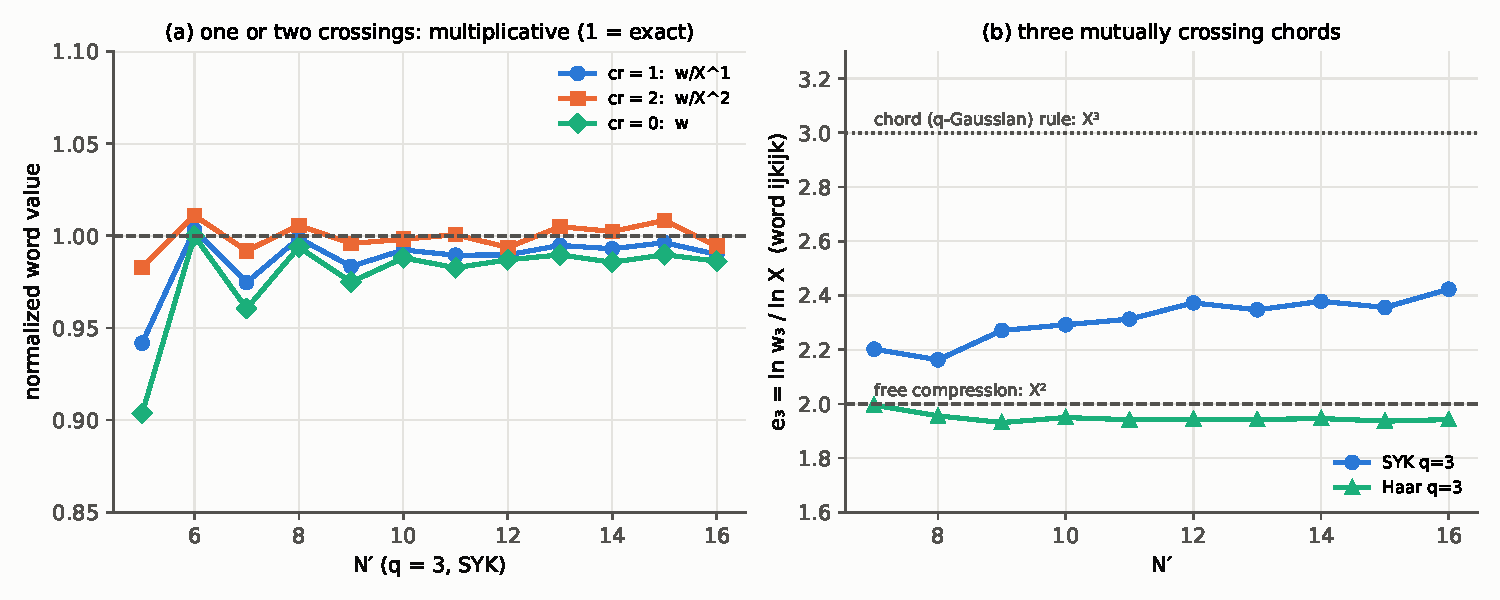
\includegraphics[width=\textwidth]{checkpoint_2026-09-28_figs/fig3_chord_rule_q3.pdf}
\caption{\NUM\ Six-letter pair words, $q=3$ SYK. (a) Words with 0, 1, 2 crossings are multiplicative in $X$.
(b) Effective exponent of the fully crossing word: Haar follows free compression ($e_3\approx2$). SYK lies between
the free and single-parameter chord rules. Error bars ($\approx0.01$) are smaller than the markers.}
\label{fig:words}
\end{figure}

%=====================================================================
\part*{Part II --- The decoder variance and the wormhole}
\addcontentsline{toc}{part}{Part II --- The decoder variance and the wormhole}
%=====================================================================

\section{The variance is a zero-energy two-point function}\label{sec:reduction}

\begin{proposition}[\DER, exact]\label{prop:reduction}
Let $\mu=\tau(\PB n_i\PB)$ and $\mathcal O=n_i-\mu$. Then
\begin{equation}
\Var(\lambda)=\frac{\Tr\,[P_j\,\mathcal O\,P_j\,\mathcal O]}{\Tr P_j}\,,\qquad
P_j\equiv\PB=\lim_{\beta\to\infty}e^{-\beta H}\Big|_{\text{charge }P},
\label{eq:reduction}
\end{equation}
with $j$ given by~\eqref{eq:jsector}.
\end{proposition}
\begin{proof}
$\Var$ is invariant under $\Pi\to1-\Pi$, so we may use $n_i$. Then
$\tau((\PB n\PB)^2)-\tau(\PB n\PB)^2=\tau(\PB n\PB n\PB)-\mu^2=\tau(\PB\,\mathcal O\,\PB\,\mathcal O\,\PB)$, since
$\PB^2=\PB$ and $\tau(\PB\mathcal O\PB)=0$. Fermion number is conserved, so $\PB$ is the zero-energy projector of the
single R-charge sector~\eqref{eq:jsector}.
\end{proof}

So $\Var(\lambda)$ is the ``infinitely-long-time'' two-point function of $\mathcal O$ in the sense of
LMRS~\cite{LMRS} (their $\hat O=POP$), with two differences:
\begin{itemize}\itemsep1pt
\item it is normalized by the number of BPS states in \emph{one} sector, $\Tr P_j$, not the total $N_{\rm BPS}$;
\item $\mathcal O$ is the \emph{same-site} bilinear $\bar\psi_i\psi_i$, not LMRS's $\psi^k\bar\psi_i$ with $i\neq k$.
\end{itemize}
At leading large $N$ the two bilinears have the same conformal two-point function,
$\langle n_i(t)n_i(0)\rangle_c=\langle\bar\psi_i(t)\psi_i(0)\rangle\langle\psi_i(t)\bar\psi_i(0)\rangle+O(1/N)$. This is
a single cross-contraction, so both have $\Delta=2\cdot\frac1{2\hat q}=\frac13$. \NUM\ In our BPS sectors,
$\Var_{\rm hop}/\Var_{n_i}=1.14,\ldots,1.06$ for $\Np=8\ldots14$, tending to 1.

%=====================================================================
\section{The super-Schwarzian answer, and why it overshoots}\label{sec:lmrs}
%=====================================================================

\subsection{Derivation from the zero-energy wavefunctions}\label{sec:mellin}
\paragraph{Imported \EST\ from LMRS~\cite{LMRS}.}
\begin{itemize}\itemsep1pt
\item The two-sided zero-energy state $\ket{Z_j}$ of $\mathcal N{=}2$ super-Liouville quantum mechanics has two fermionic
  components, $g_{1,2}\propto e^{-\ell/2}K_{\frac12\mp j}(2e^{-\ell/2})$ (their eq.~22), normalizable for $|j|<\frac12$.
\item A neutral matter operator of dimension $\Delta$ acts on it as multiplication by $e^{-\Delta\ell}$ (their eq.~54).
\item The $\beta\to\infty$ two-sided state in sector $j$ is $A_{z,j}\ket{Z_j}$ (their eqs.~37, 39).
\end{itemize}

\paragraph{Step 1 \DER: reduction to a normalized expectation value.}
$\Tr[P_j\hat O P_j\hat O]=|A_{z,j}|^2\langle Z_j|e^{-\Delta\ell}|Z_j\rangle$. At $\Delta=0$ this must equal
$\Tr P_j$, so
\begin{equation}
\frac{\Tr[P_j\hat O P_j\hat O]}{\Tr P_j}=\frac{\langle Z_j|e^{-\Delta\ell}|Z_j\rangle}{\langle Z_j|Z_j\rangle}\,.
\label{eq:normexp}
\end{equation}
Neither $\eS$ nor the TFD coefficient enters; only the shape of the wavefunction does.

\paragraph{Step 2 \DER: a Mellin integral.} For a neutral operator the $U(1)$ integral is trivial. With $x=2e^{-\ell/2}$
($d\ell=-2dx/x$, $e^{-\ell}=x^2/4$, $e^{-\Delta\ell}=(x/2)^{2\Delta}$),
\[
I_\nu(\Delta)\equiv\int_{-\infty}^{\infty}\!d\ell\;e^{-(1+\Delta)\ell}K_\nu(2e^{-\ell/2})^2=2^{-1-2\Delta}\!\int_0^\infty\!x^{1+2\Delta}K_\nu(x)^2\,dx .
\]
Use the Mellin transform (Gradshteyn--Ryzhik 6.576.4 with equal arguments~\cite{GR}; checked numerically to $10^{-11}$):
\[
\int_0^\infty x^{s-1}K_\nu(x)^2dx=\frac{\sqrt\pi\,\Gamma(\frac s2)\Gamma(\frac s2-\nu)\Gamma(\frac s2+\nu)}{4\,\Gamma(\frac{s+1}2)},\qquad \operatorname{Re}s>2|\nu| .
\]
Set $s=2+2\Delta$ and sum the two components $\nu=\frac12\mp j$. Using $\Gamma(z+1)=z\Gamma(z)$ on the second factors,
\[
\Gamma(\Delta{+}\tfrac12{+}j)\Gamma(\Delta{+}\tfrac32{-}j)+\Gamma(\Delta{+}\tfrac12{-}j)\Gamma(\Delta{+}\tfrac32{+}j)
=(2\Delta+1)\,\Gamma(\Delta{+}\tfrac12{+}j)\Gamma(\Delta{+}\tfrac12{-}j).
\]
Then $(2\Delta+1)/\Gamma(\Delta+\frac32)=2/\Gamma(\Delta+\frac12)$, and Legendre duplication,
$\Gamma(\Delta)\Gamma(\Delta+\frac12)=2^{1-2\Delta}\sqrt\pi\,\Gamma(2\Delta)$, give
\begin{equation}
\mathcal N_j(\Delta)\equiv I_{\frac12-j}+I_{\frac12+j}
=\frac18\,\frac{\Delta\,\Gamma(\Delta)^2\,\Gamma(\Delta+\frac12+j)\Gamma(\Delta+\frac12-j)}{\Gamma(2\Delta)} .
\label{eq:Nj}
\end{equation}
The convergence condition at $\Delta=0$ is exactly $|j|<\frac12$, the normalizability condition of $\ket{Z_j}$.

\paragraph{Step 3 \DER: normalize.}
$\mathcal N_j(0)=\frac14\Gamma(\frac12+j)\Gamma(\frac12-j)=\pi/(4\cos\pi j)$. This reproduces the norm
$\langle Z_j|Z_j\rangle\propto1/\cos\pi j$ of~\cite[eq.~26]{LMRS}, a check on Step 2. Hence
\begin{equation}
\langle e^{-\Delta\ell}\rangle_j=\frac{\cos\pi j}{2\pi}\,\frac{\Delta\,\Gamma(\Delta)^2\,\Gamma(\Delta+\frac12\pm j)}{\Gamma(2\Delta)}
\equiv F(\Delta,j),
\label{eq:Fdj}
\end{equation}
which is exactly LMRS eq.~(66) divided by $\Tr P_j=\eS\cos\pi j$.

\paragraph{Step 4 \EST: SYK normalization.}
Converting from Schwarzian to SYK units multiplies by $b_{\hat q}^2(2CJ)^{-2\Delta}$, with
$b_{\hat q}=[\tan(\pi/2\hat q)/2\pi]^{1/\hat q}$ and $C=\alpha_SN/J$, $\alpha_S=0.00842$ for $\hat q=3$
(LMRS eqs.~64, 78--80). Therefore
\begin{equation}
\boxed{\;r_{\rm LMRS}(\Np)=\frac{b_{\hat q}^2\,(2\alpha_S\Np)^{-2/3}\,F(\tfrac13,j)}{b(1-b)}\;}
\label{eq:rlmrs}
\end{equation}
with no free parameter.
\begin{itemize}\itemsep1pt
\item Checks: the code reproduces the LMRS Table~1 Schwarzian column (0.1112 vs 0.111; 0.0874 vs 0.0874); $F(0,j)=1$;
  $J$ cancels.
\item Note: LMRS eq.~(77) prints $\langle C\bar C\rangle=2J/N$. FGMS~\cite[eq.~5.4]{FGMS} has $2J/N^2$, which is
  required for extensivity. This matters only for gap-based checks.
\end{itemize}

\subsection{Comparison}\label{sec:lmrscomp}
\begin{table}[h]\centering\small
\begin{tabular}{@{}lccccccccc@{}}\toprule
$\Np$ & 9 & 10 & 11 & 12 & 13 & 14 & 15 & 16\\\midrule
$r$ (SYK) & 0.728 & 0.746 & 0.666 & 0.687 & 0.617 & 0.642 & 0.577 & 0.601\\
$r_{\rm LMRS}$ & 0.957 & 0.957 & 0.833 & 0.847 & 0.744 & 0.765 & 0.675 & 0.700\\
Haar $r=a$ & 0.643 & 0.643 & 0.526 & 0.526 & 0.425 & 0.425 & 0.340 & 0.340\\\bottomrule
\end{tabular}
\caption{\NUM\ Decoder variance ratio against the parameter-free super-Schwarzian prediction~\eqref{eq:rlmrs}.}
\label{tab:lmrs}
\end{table}

\paragraph{What works \NUM.}
\begin{itemize}\itemsep1pt
\item \textbf{Parity.} The $j$-factor $F(\frac13,-\frac16)/F(\frac13,0)=\cos\frac\pi6\,\Gamma(1)\Gamma(\frac23)/\Gamma(\frac56)^2=0.920$
  removes the even/odd alternation of $r$ with no parameters.
\item \textbf{A pre-registered test} at fixed even $\Np$, comparing the $j=\pm\frac13$ sectors ($P=\Np/2\pm1$) with
  $j=0$. Predicted $\Var_{1/3}/\Var_0=\frac12\Gamma(\frac76)\Gamma(\frac12)/\Gamma(\frac56)^2=0.645$. Measured:
  $0.642,0.668,0.677,0.683$ ($\Np=8\ldots14$). The Haar value is $0.586\to0.560$, and ``no $j$-dependence'' gives 1.
  So this is a 6\,\% success, although the measured ratio drifts away from the prediction.
\end{itemize}

\paragraph{What fails \NUM.} The magnitude is too high by 15--60\,\%. The $\Np$-dependence also does not match:
the pure $\Np^{-2/3}$ shape with free normalization gives $\chi^2/\text{dof}=335$. A fitted $1-2.2/\Np$ factor
restores agreement, but so does a plain power $\Np^{-0.44}$. That fitted factor is not a prediction.

\subsection{Diagnosis: no conformal window \DER}
By Steps 1--4, the prediction is the zero-energy average of the conformal matter correlator
$b_{\hat q}^2(Jt)^{-2\Delta}$ with $Jt(\ell)=2\alpha_S\Np e^{\ell/2}$. The weight $\rho_j(\ell)e^{-\Delta\ell}$ fixes
which physical times dominate:

\begin{center}\small
\begin{tabular}{@{}lccccc@{}}\toprule
$\Np$ & 10 & 15 & 20 & 50 & 120\\\midrule
median $Jt$ & 0.50 & 0.75 & 1.0 & 2.5 & 6.0\\
weight where conformal value $>$ UV maximum $\frac14$ & 67\,\% & 49\,\% & 35\,\% & 4\,\% & 0\\\bottomrule
\end{tabular}
\end{center}

At our sizes the ``zero-energy'' correlator is dominated by times \emph{shorter than} $1/J$. There the conformal
input overshoots the true correlator, which is bounded by its equal-time value. The effective small parameter is
$1/(2\alpha_S\Np)\approx60/\Np$, and a clean window needs $\Np\sim10^2$. \NUM\ Consistent with this: the BPS gap is
$0.19J$ at $\Np=14$ (not $\ll J$), and $r_{\rm LMRS}>1$ for $\Np\le8$. A parameter-free toy that caps the conformal
correlator at its UV value brings the prediction within 0--10\,\% of the data, for two different operators.

%=====================================================================
\section{The finite-$\lambda$ super-chord answer}\label{sec:chord}
%=====================================================================

The double-scaled theory ($N,p\to\infty$ with $\lambda=2p^2/N$ fixed, $q=e^{-\lambda}$) is solvable by chord methods and
is UV-complete. The super-Schwarzian is its triple-scaling limit $\lambda\to0$~\cite{BLY}. Boruch, Lin and Yan
construct the two-sided super-chord Hilbert space (chord number $n$ = discrete wormhole length, $\ell=2\lambda n$) and
its zero-energy Hartle--Hawking state $\ket{\Psi,j}$ (\EST, their eqs.~3.1--3.11). They compute the normalized
zero-temperature two-point function of a neutral operator (\EST, their eqs.~4.5--4.8):
\begin{equation}
\frac{\langle\Psi,j|q^{2\Delta n}|\Psi,j\rangle}{\langle\Psi,j|\Psi,j\rangle}
=\frac{(q^{2+4\Delta};q^2)_\infty\,(q^{1\pm2j};q^2)_\infty\,(q^2;q^2)_\infty}{(q^{2+2\Delta};q^2)_\infty^2\,(q^{1+2\Delta\pm2j};q^2)_\infty}\,.
\label{eq:bly48}
\end{equation}
As $\lambda\to0$ this tends to $(2\lambda)^{2\Delta}F(\Delta,j)$, i.e.\ to~\eqref{eq:Fdj} (checked: ratio $1-3\times10^{-3}$ at
$\lambda=0.3$).

\paragraph{Identification with $r$ \DER.} BLY normalize the matter operator so that $W_LW_R\propto q^{\Delta(n_O+n_X)}$ with
unit constant, i.e.\ its infinite-temperature two-point function in the charge sector equals 1. Since
$\ket{\Psi,j}\propto\Pi_{0,j}\ket{\Omega,j}$, eq.~\eqref{eq:bly48} equals
$[\Tr(P_jWP_jW)/\Tr P_j]/[\Tr_j(WW)/\Tr_j\mathbb 1]$. For $W=n_i-\mu$ on $\Lambda^P$, the denominator is exactly
$b(1-b)$. By Proposition~\ref{prop:reduction},
\begin{equation}
\boxed{\;r=\text{eq.~\eqref{eq:bly48}}\Big|_{\lambda=2p^2/\Np,\ \Delta=1/p,\ j=(P-\Np/2)/p}\;}
\label{eq:rchord}
\end{equation}
Here $\Delta=1/p$ because $\bar\psi_i\psi_i$ has one $\psi$ and one $\bar\psi$ (BLY eq.~1.8). No conformal
normalization and no $\alpha_S$ enter.

\begin{table}[h]\centering\small
\begin{tabular}{@{}ccc cccc cc@{}}\toprule
$\Np$ & $j$ & $\lambda$ & $r$ (SYK) & $r$ chord & $r_{\rm LMRS}$ & SYK/chord & $a$ exact & $a$ chord\\\midrule
6 & 0 & 3.00 & 0.905 & 0.913 & 1.345 & 0.990 & 0.900 & 0.900\\
8 & 0 & 2.25 & 0.819 & 0.832 & 1.110 & 0.984 & 0.771 & 0.789\\
10 & 0 & 1.80 & 0.746 & 0.756 & 0.957 & 0.987 & 0.643 & 0.671\\
12 & 0 & 1.50 & 0.687 & 0.690 & 0.847 & 0.996 & 0.526 & 0.559\\
13 & $-\frac16$ & 1.38 & 0.617 & 0.613 & 0.744 & 1.007 & 0.425 & 0.456\\
14 & 0 & 1.29 & 0.642 & 0.635 & 0.765 & 1.011 & 0.425 & 0.459\\
15 & $-\frac16$ & 1.20 & 0.577 & 0.565 & 0.675 & 1.021 & 0.340 & 0.371\\
16 & 0 & 1.13 & $0.601\pm0.005$ & 0.589 & 0.700 & 1.022 & 0.340 & 0.373\\
14 & $-\frac13$ & 1.29 & 0.449 & 0.418 & 0.504 & 1.074 & 0.243 & 0.265\\\bottomrule
\end{tabular}
\caption{\NUM\ Exact $q=3$ SYK against the parameter-free finite-$\lambda$ prediction~\eqref{eq:rchord}. The BPS
fraction is from the exact index~\eqref{eq:index} and from the double-scaled formula $D(j)$~\cite[eq.~3.17]{BLY}.}
\label{tab:chord}
\end{table}

\paragraph{Results \NUM.}
\begin{itemize}\itemsep1pt
\item $r$ agrees within $2.2\,\%$ for every $\Np=5\ldots16$, including parity, with no rescaling
  (Fig.~\ref{fig:chord}). The super-Schwarzian misses by 15--60\,\% over the same range.
\item There is a small systematic drift in SYK/chord ($0.98\to1.02$). In the $j=\pm\frac13$ sectors the agreement
  degrades to $+7\,\%$ at $\Np=14$.
\item The double-scaled BPS fraction overshoots the exact one by up to 10\,\%. This is a pure finite-$p$ effect:
  $\cos^{\Np}(\pi/2p)$ versus $e^{-\Np\pi^2/8p^2}$.
\end{itemize}

\paragraph{Caveats.}
\begin{itemize}\itemsep1pt
\item The $\lambda$ identification is BLY's standard $\lambda=2p^2/N$, fixed before comparing. The prediction
  scales as $r\propto\lambda^{0.4\text{--}0.6}$, so a 5\,\% ambiguity in $\lambda$ moves $r$ by about 2.5\,\%. The
  2\,\% agreement is at the resolution of the double-scaled mapping at $p=3$.
\item The double-scaled theory at $\lambda=18/\Np$ is not the $\Np\to\infty$ limit at fixed $p=3$. Its Schwarzian
  coupling is $\alpha_S=1/(8p^2)=0.0139$ versus $0.00842$. Agreement must eventually degrade at large $\Np$; the
  positive drift may be its onset.
\end{itemize}

\paragraph{Interpretation \INTERP.} Together with the diagnosis above: at accessible sizes the decoder variance sits in a
\emph{double-scaled} regime ($\lambda\approx1.1$--$3.6$), not a Schwarzian one. The chord theory, as the UV
completion, captures the crossover the Schwarzian misses. BLY draw the same lesson for the ground-state
degeneracy itself.

\begin{figure}[t]
\centering
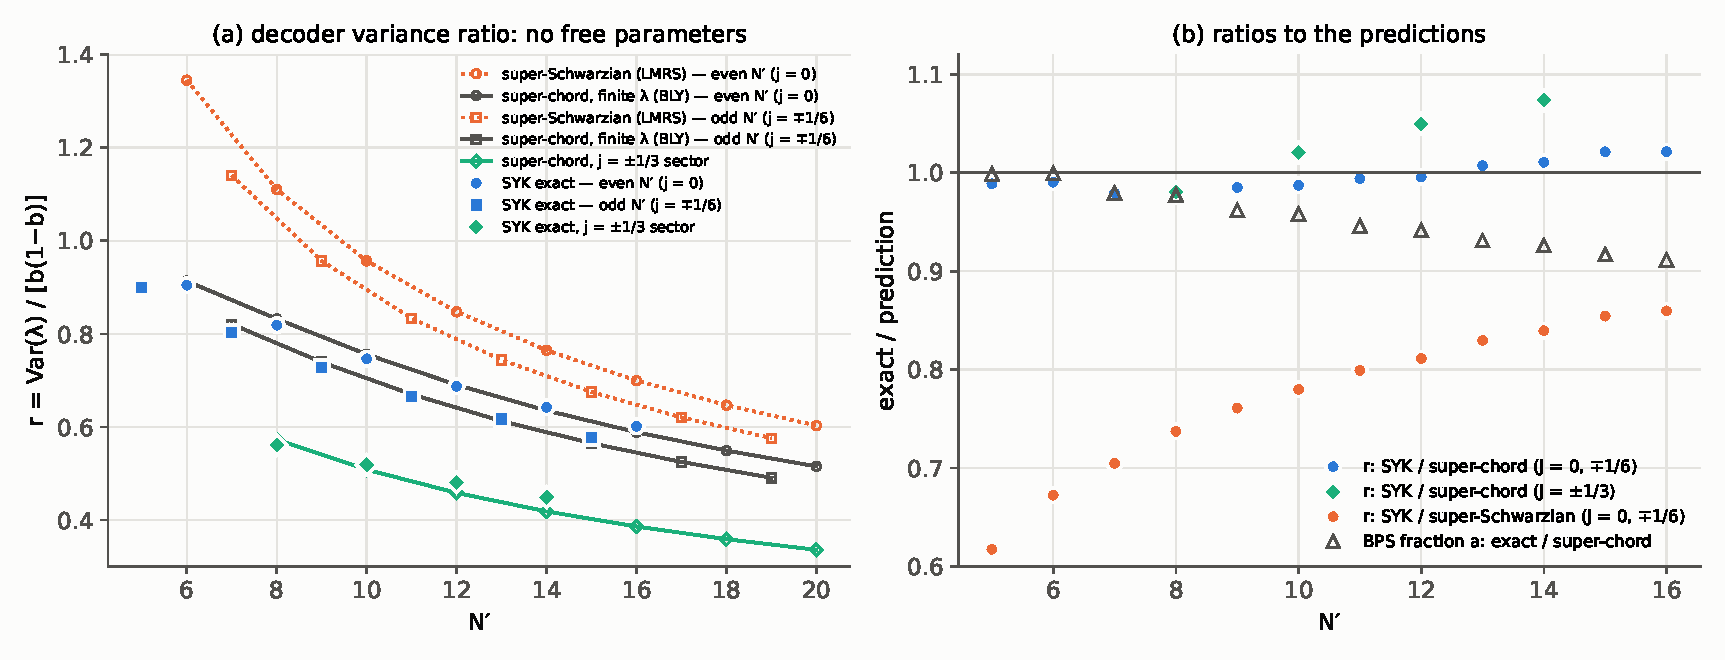
\includegraphics[width=\textwidth]{checkpoint_2026-09-28_figs/fig_r_a_vs_chords.pdf}
\caption{\NUM\ (a) $r$ versus $\Np$: exact SYK (filled), finite-$\lambda$ super-chord (solid; eq.~\ref{eq:rchord}),
super-Schwarzian (dotted; eq.~\ref{eq:rlmrs}); no free parameters. (b) Ratios to the predictions, including the
BPS fraction $a$.}
\label{fig:chord}
\end{figure}

%=====================================================================
\section{Deviation from freeness $=$ wormholes of nonzero length}\label{sec:freeness}
%=====================================================================

The project's framing asks for ``the deviation from freeness'' of the decoder law. The chord theory gives this
deviation a precise geometric meaning, at least for the second free cumulant.

\subsection{Two facts about the same distribution}
Let $P_n$ be the probability that the supersymmetric wormhole $\ket{\Psi,j}$ has chord number $n$. It is the
$n$-sector weight of $\ket{\Psi,j}$, normalized by eq.~3.11 of~\cite{BLY}; different $n$ are orthogonal.

\paragraph{Fact 1: the BPS fraction is the zero-length probability \EST\ \cite[eqs.~1.1, 3.12--3.15]{BLY}.}
Slice the fixed-charge partition function two-sidedly:
$Z(j,\beta)/Z(j,0)=\langle\Omega,j|e^{-\beta H}|\Omega,j\rangle/\langle\Omega,j|\Omega,j\rangle$, where $\ket{\Omega,j}$
is the empty ($n=0$) wormhole. As $\beta\to\infty$, $e^{-\beta H}$ projects onto the chord ground state:
\begin{equation}
a=\frac{d}{D}=\frac{Z(j,\infty)}{Z(j,0)}=\frac{|\langle\Omega,j|\Psi,j\rangle|^2}{\langle\Omega,j|\Omega,j\rangle\langle\Psi,j|\Psi,j\rangle}=P_0 .
\label{eq:aP0}
\end{equation}

\paragraph{Fact 2: $r$ is the propagator averaged over wormhole lengths \DER.} By~\eqref{eq:rchord} and
$W_LW_R=q^{2\Delta n}$ on empty wormholes (a scalar on each $n$-sector),
\begin{equation}
r=\sum_{n\ge0}P_n\,q^{2\Delta n}.
\label{eq:rPn}
\end{equation}

\subsection{The identity}
Since $q^{2\Delta\cdot0}=1$, facts~\eqref{eq:aP0}--\eqref{eq:rPn} combine into
\begin{equation}
\boxed{\;r=\underbrace{a}_{\text{Haar / Wachter, eq.~\eqref{eq:rhaar}}}+\sum_{n\ge1}P_n\,q^{2\Delta n},\qquad
\eta_r\equiv\frac{r-a}{1-a}=\big\langle q^{2\Delta n}\big\rangle_{n\ge1}\;}
\label{eq:identity}
\end{equation}
\DER\ Verified from the Hartle--Hawking recursion (BLY eqs.~3.2--3.11) for $\Np=8,12,14,16$:
$\sum_nP_n=1$, $P_0=D(j)$, and $\sum_nP_nq^{2n/3}$ equals~\eqref{eq:bly48} to $10^{-10}$ or better
(\path{hh_length_distribution}, test \path{test_free_compression_is_zero_length_term}).

\paragraph{Reading \INTERP.}
\begin{itemize}\itemsep1pt
\item The free-probability value of the second free cumulant, $\rho_2=a$, is \emph{exactly} the contribution of the
  zero-length wormhole.
\item The deviation from freeness, $r-a\ge0$, is the contribution of wormholes of nonzero length, each weighted
  by the matter propagator $q^{2\Delta n}=e^{-\Delta\ell}$.
\item The rigidity fraction $\eta_r$ is the propagator averaged over nonzero-length wormholes.
\item In particular $r\ge a$ is automatic in the chord theory. \NUM\ The realization-averaged $r$ satisfies it
  within errors at every $(q,\Np)$ measured, and by many standard errors for $q=3$, $\Np\ge7$ (e.g.\ $r/a=1.77$
  at $\Np=16$). Individual realizations violate it only where $a\gtrsim0.9$ and $d$ is tiny ($q=3$, $\Np=5,6$;
  $q=5$, $\Np=9,10$; 2 of 300 at $q=3$, $\Np=7$). There $r\approx a$ and sample fluctuations cross; the minimum
  single-realization $r/a$ is $0.965$.
\end{itemize}
Figure~\ref{fig:worm}(a) shows the decomposition at $\Np=14$: $a=P_0=0.459$ of $r=0.635$ comes from $n=0$, and the
remaining $0.176$ from $n=1,2,3,\ldots$

\begin{figure}[t]
\centering
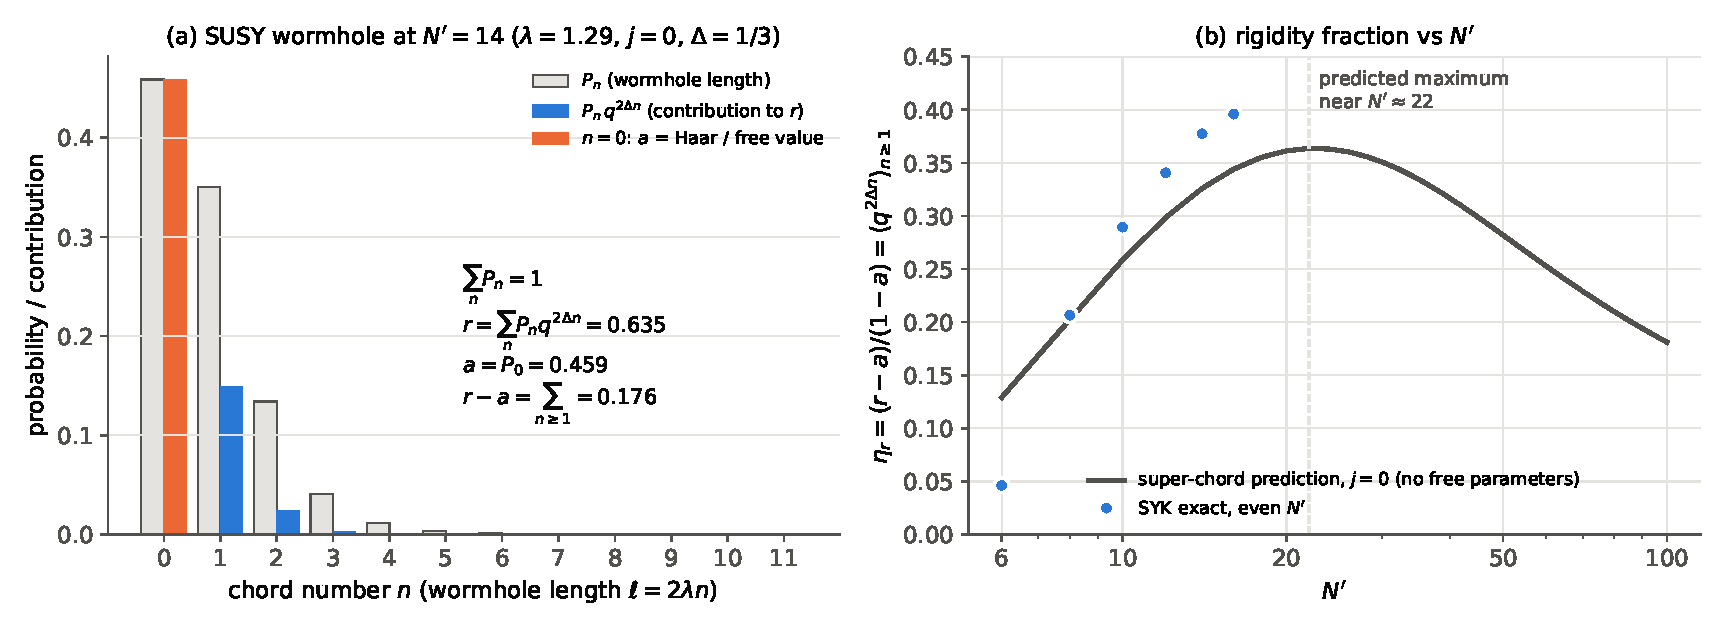
\includegraphics[width=\textwidth]{checkpoint_2026-09-28_figs/fig_wormhole_freeness.pdf}
\caption{(a) \DER\ Wormhole-length distribution $P_n$ of the supersymmetric Hartle--Hawking state at $\Np=14$
($\lambda=18/14$, $j=0$) and its contribution $P_nq^{2\Delta n}$ to $r$. The $n=0$ bar is the BPS fraction $a$, the
entire Haar/free value. (b) \NUM\ vs prediction: $\eta_r$ from the chord theory (line; no parameters) and exact SYK
(points). The chord curve peaks near $\Np\approx22$. The measured values lie about $0.04$ above it, consistent with the
finite-$p$ excess of $a_{\rm chord}$ over the exact $a$. At $\Np=6$, $1-a=0.1$, so $\eta_r$ is poorly conditioned.}
\label{fig:worm}
\end{figure}

\subsection{Consequences}
\begin{enumerate}\itemsep2pt
\item \textbf{$\eta_r$ turns over} \NUM/\INTERP. In the chord theory $\eta_r$ \emph{peaks} near $\Np\approx22$
  ($\eta_r\approx0.36$) and then decays. The measured deceleration ($0.34\to0.38\to0.40$ at $\Np=12,14,16$) is the
  approach to this maximum, not a plateau. This is a sharp, testable prediction for $\Np\gtrsim20$ (stochastic
  trace estimation). The turnover is robust beyond the double-scaled approximation: at fixed $p=3$, LMRS also
  gives $r\propto\Np^{-2/3}\to0$.
\item \textbf{Q1 settled structurally.} $a\sim e^{-\pi^2\Np/72}$ in the chord theory (exactly, at $p=3$,
  $a\propto\cos^{\Np}(\pi/6)$ up to the binomial normalization) is exponentially small, while
  $r\sim\lambda^{2\Delta}\propto\Np^{-2/3}$ is power-law small. So $r/a\to\infty$: the decoder law moves ever further
  from Wachter, while $r\to0$ (ever further from the commuting UV).
\item \textbf{Conjecture} \CONJ. The \emph{entire} free-compression (Wachter/MANOVA) law is the zero-length truncation
  of the super-chord computation of the decoder moments. Only $m_2$ has been tested.
\end{enumerate}

%=====================================================================
\section{Open problems and next steps}
%=====================================================================
\begin{enumerate}\itemsep2pt
\item \textbf{Zero-temperature OTOC: $X$ and $e_3$.} BLY \S5 constructs one-particle wormholes and the operator
  $W_LW_R\sim q^{\Delta(n_O+n_X)_{\rm tot}}$ (their eq.~5.18), but does not evaluate the zero-temperature OTOC. For our
  operators the matter--matter crossing weight must be site-local: 1 for disjoint sites, since those bilinears
  commute, rather than the random-operator $q^{\Delta^2}$. This gives a parameter-free prediction of
  $X\approx0.73$--$0.85$ and $e_3\approx2.3$--$2.4$ (Table~\ref{tab:campaign}).
\item \textbf{Higher moments and the density.} $m_k=\tau(O^k)$ are zero-temperature $k$-point functions of \emph{one
  fixed projector}. Writing $n_i=\bar\psi_i\psi_i$ with $\psi_i$ a single-fermion chiral chord restores a Wick
  structure, because the infinite-temperature state is Gaussian. Same-site fermion chords then cross with a sign.
  Testing the conjecture above requires these.
\item \textbf{Finite-$p$ corrections.} Explain the $\pm2\,\%$ drift and the $j=\pm\frac13$ deviation. Candidates: exact
  finite-$N$ intersection weights (e.g.\ $1-2p/N$ vs $e^{-2p/N}$ for a single-site bilinear crossing a 3-body
  chord), and the $\lambda$ identification.
\item \textbf{Larger $\Np$.} Test the $\eta_r$ maximum near $\Np\approx22$ and the breakdown of double scaling.
\item \textbf{Framing.} The project overview's ``planar chords $=$ non-crossing partitions (Narayana) $\Rightarrow$
  Wachter'' does not describe the actual $\mathcal N{=}2$ chord rules. Those have directed chords, friend/enemy
  weights and $q^\Delta$ matter weights, and give Wachter only as the zero-length piece.
\end{enumerate}

\appendix
\section{Reproducibility}
All numbers are exact linear algebra (no stochastic trace estimation), with the same coupling generator and seeds
as \path{src/decoder_fast.py}. Code state: commit \texttt{081877d} plus the working-tree files added for this note
(\path{src/dssyk_n2.py} [\path{hh_length_distribution}], \path{scripts/plot_wormhole_freeness.py}).

\begin{center}\small
\begin{tabular}{@{}p{0.33\textwidth}p{0.62\textwidth}@{}}\toprule
Item & Code / data\\\midrule
Chord invariants, Tab.~\ref{tab:campaign}, Fig.~\ref{fig:words} & \path{scripts/run_chord_invariants.py},
\path{scripts/chord_invariants_campaign.sh} (groups A--F2), \path{scripts/analyze_chord_invariants.py};
\path{results/data/chord_invariants_2026-09-28/} (JSONL per realization, \path{meta_*.json} with args and commit)\\
Super-Schwarzian, Tab.~\ref{tab:lmrs} & \path{src/lmrs_predictions.py}, \path{scripts/compare_lmrs_variance.py},
\path{scripts/lmrs_mismatch_checks.py}, \path{scripts/lmrs_jsector_test.py}; \path{results/data/lmrs_variance_2026-09-28/}\\
Super-chord, Tab.~\ref{tab:chord}, Figs.~\ref{fig:chord}--\ref{fig:worm} & \path{src/dssyk_n2.py},
\path{scripts/compare_dssyk.py}, \path{scripts/plot_wormhole_freeness.py}; \path{results/data/dssyk_2026-09-28/}\\
Tests & \path{tests/test_chord_invariants.py}, \path{tests/test_lmrs_predictions.py}, \path{tests/test_dssyk_n2.py}\\
Derivations (living) & \path{docs/derivations.md} D1, D2\\\bottomrule
\end{tabular}
\end{center}

\paragraph{Realizations.} $q=3$: 60/30 (SYK/Haar) at $\Np=5$--8; 40/20 at 9--10; 24/12 at 11; 16/8 at 12; 10/5 at 13;
4/2 at 14; 3/2 at 15; 2/1 at 16. $q=5$: 20/10 at 9--14; 8/4 at 15; 4/2 at 16; 2/1 at 17. $j$-sector test: seeds
0--3, $\Np=8$--14.

\paragraph{Memory safety.} The two largest runs ($q=3$, $\Np=16$; $q=5$, $\Np=17$) were OOM-killed once when run
concurrently. They were rerun after two changes: a partial eigendecomposition of $\{Q,Q^\dagger\}$ with a
certified spectral gap, and a byte-bounded cache. Regression against stored rows: $\le4\times10^{-16}$. All heavy
jobs now run under \path{scripts/memwatch.py} (per-job cap, 30\,GB project budget). Peaks were 7.5 and 7.0\,GB.

\begin{thebibliography}{9}\small
\bibitem{CV} J.~Chryssanthacopoulos and D.~Vegh, \emph{Fortuity and fragility in supersymmetric SYK}, arXiv:2608.12160 (2026).
\bibitem{FGMS} W.~Fu, D.~Gaiotto, J.~Maldacena and S.~Sachdev, \emph{Supersymmetric Sachdev-Ye-Kitaev models}, Phys.\ Rev.\ D \textbf{95} (2017) 026009, arXiv:1610.08917.
\bibitem{LMRS} H.~W.~Lin, J.~Maldacena, L.~Rozenberg and J.~Shan, \emph{Looking at supersymmetric black holes for a very long time}, SciPost Phys.\ \textbf{14} (2023) 128, arXiv:2207.00408.
\bibitem{BLY} J.~Boruch, H.~W.~Lin and C.~Yan, \emph{Exploring supersymmetric wormholes in $\mathcal N=2$ SYK with chords}, arXiv:2308.16283 (2023).
\bibitem{NS} A.~Nica and R.~Speicher, \emph{Lectures on the Combinatorics of Free Probability}, London Math.\ Soc.\ Lecture Note Series 335, Cambridge University Press (2006).
\bibitem{Kunisky} D.~Kunisky, \emph{Generic MANOVA limit theorems for products of projections}, arXiv:2301.09543 (2023).
\bibitem{GR} I.~S.~Gradshteyn and I.~M.~Ryzhik, \emph{Table of Integrals, Series, and Products}, Academic Press, formula 6.576.4.
\end{thebibliography}

\end{document}
